\chapter{Results and Discussion}
For this particular project 2 Datasets have been used for training namely: 
\begin{itemize}
    \item \href{https://www.kaggle.com/navoneel/brain-mri-images-for-brain-tumor-detection}{Brain MRI Images for Brain Tumor Detection}
    \item \href{https://www.kaggle.com/ahmedhamada0/brain-tumor-detection}{Br35H :: Brain Tumor Detection 2020}
\end{itemize}
However Dataset 1 is a small dataset, There were not enough examples to train the neural network. Hence Data augmentation, was performed on Dataset 1. Data augmentation also is useful in taclking the data imbalance issue in the data. With this updated Dataset we merged both of these Datasets(Augmented dataset1 and dataset2) into a single final dataset. All this data was then passed onto a final dataset, which was then separated into 3 segments: Train , Test and Validation in ratio of 70:15:15. Then these train images were passed on to the model. The model then was trained for 6 times. Each version trained had a different parameter associated with it. These parameters and results associated with each result can be understood in the section \ref{section:results}.
Based on the results from each verion the highest accuracy achieved is 100\%. However the loss associated with that version suggests overfitting. Overfitting according to \href{https://en.wikipedia.org/wiki/Overfitting}{Wikipedia} is "the production of an analysis that corresponds too closely or exactly to a particular set of data, and may therefore fail to fit additional data or predict future observations reliably".Hence, the next best version with an accuracy of 92\% is taken into consideration for further development. This final model was then manually tested with a \href{https://www.kaggle.com/preetviradiya/brian-tumor-dataset}{third dataset}, to test the accuracy of the model. The Model is efficiently able to classify MRI Scan into Tumorous and Non Tumorous Image Respectively.

\section{Dataset Information}
Table 5.1 displays the number of imgaes in each dataset before augmentation\\
\begin{table}[h!]
\caption{Contents of dataset before augmentation}
\label{tab:table1}
\begin{tabular}{|c|c|c|}
\hline
\rowcolor[HTML]{CBCEFB} 
\textbf{Dataset} & \textbf{Tumorous Images} & \textbf{Non Tumorous Images} \\ \hline
Dataset 1        & 155                      & 98                           \\ \hline
Dataset 2        & 1500                     & 1500                         \\ \hline
Dataset 3        & 2513                     & 2087                         \\ \hline
\end{tabular}
\end{table}

Table 5.2 displays the number of imgaes in each dataset after augmentation\\
\begin{table}[h!]
\caption{Contents of dataset after augmentation}
\label{tab:table1}
\begin{tabular}{|c|c|c|}
\hline
\rowcolor[HTML]{CBCEFB} 
\textbf{Dataset} & \textbf{Tumorous Images} & \textbf{Non Tumorous Images} \\ \hline
Dataset 1        & 1083                      & 980                           \\ \hline
Dataset 2        & 1500                     & 1500                         \\ \hline
Dataset 3        & 2513                     & 2087                         \\ \hline
\end{tabular}
\end{table}

Table 5.3 displays the number of imgaes in the final dataset after merging\\
\begin{table}[h!]
\caption{Contents of final dataset}
\label{tab:table1}
\begin{tabular}{|c|c|c|}
\hline
\rowcolor[HTML]{CBCEFB} 
\textbf{Dataset} & \textbf{Tumorous Images} & \textbf{Non Tumorous Images} \\ \hline
Final Dataset    & 2583                     & 2480                         \\ \hline
\end{tabular}
\end{table}

\section{Training Results}
\label{section:results}
As part of model training different approaches were considered. Some of the main parameters into consideration are as follows:
\begin{itemize}
    \item Amount of images used.
    \item Transfer learning.
    \item Creating callbacks to prevent overtraining.
\end{itemize}
Table below highlights the different results obtained with each version alongwith the parameter changes performed.\\
% Please add the following required packages to your document preamble:
% \usepackage{multirow}
% \usepackage{graphicx}
% \usepackage[table,xcdraw]{xcolor}
% If you use beamer only pass "xcolor=table" option, i.e. \documentclass[xcolor=table]{beamer}
% Please add the following required packages to your document preamble:
% \usepackage{multirow}
% \usepackage{graphicx}
% \usepackage[table,xcdraw]{xcolor}
% If you use beamer only pass "xcolor=table" option, i.e. \documentclass[xcolor=table]{beamer}
% Please add the following required packages to your document preamble:
% \usepackage{multirow}
% \usepackage{graphicx}
% \usepackage[table,xcdraw]{xcolor}
% If you use beamer only pass "xcolor=table" option, i.e. \documentclass[xcolor=table]{beamer}
\begin{table}[h!]
\caption{Results obtained from each version}
\label{tab:table1}
\resizebox{\textwidth}{!}{%
\begin{tabular}{|c|cc|c|c|c|c|c|}
\hline
\rowcolor[HTML]{CBCEFB} 
\cellcolor[HTML]{CBCEFB}                             & \multicolumn{2}{c|}{\cellcolor[HTML]{CBCEFB}Number of Images Used}   & \cellcolor[HTML]{CBCEFB}                                                                       & \cellcolor[HTML]{CBCEFB}                                                                                         & \cellcolor[HTML]{CBCEFB}                            & \cellcolor[HTML]{CBCEFB}                                & \cellcolor[HTML]{CBCEFB}                                                                                                                                                                             \\ \cline{2-3}
\rowcolor[HTML]{CBCEFB} 
\multirow{-2}{*}{\cellcolor[HTML]{CBCEFB}Version \#} & \multicolumn{1}{c|}{\cellcolor[HTML]{CBCEFB}Tumorous} & Non-Tumorous & \multirow{-2}{*}{\cellcolor[HTML]{CBCEFB}\begin{tabular}[c]{@{}c@{}}Model\\ Type\end{tabular}} & \multirow{-2}{*}{\cellcolor[HTML]{CBCEFB}\begin{tabular}[c]{@{}c@{}}No. of Datasets \\ Implemented\end{tabular}} & \multirow{-2}{*}{\cellcolor[HTML]{CBCEFB}Test Loss} & \multirow{-2}{*}{\cellcolor[HTML]{CBCEFB}Test Accuracy} & \multirow{-2}{*}{\cellcolor[HTML]{CBCEFB}\begin{tabular}[c]{@{}c@{}}Additional Parameters/\\ Notes\end{tabular}}                                                                                     \\ \hline
\#1                                                  & \multicolumn{1}{c|}{155}                              & 98           & \begin{tabular}[c]{@{}c@{}}CNN:\\ InceptionResNetV2\end{tabular}                               & 1(Dataset 1)                                                                                                     & 0.4165                                              & 0.7692                                                  & \begin{tabular}[c]{@{}c@{}}Transfer Learning on \\ InceptionResNetV2\end{tabular}                                                                                                                    \\ \hline
\#2                                                  & \multicolumn{1}{c|}{1083}                             & 980          & \begin{tabular}[c]{@{}c@{}}CNN:\\ InceptionResNetV2\end{tabular}                               & \begin{tabular}[c]{@{}c@{}}2(Dataset 1, and\\ Augmented)\end{tabular}                                            & 0.0351                                              & 1                                                       & \begin{tabular}[c]{@{}c@{}}1) Transfer Learning on \\ InceptionResNetV2\\ 2) Data imbalance resolved\\ 3)Overfitting observed. Huge gap\\ observed between Train and\\ Validation loss.\end{tabular} \\ \hline
\#3                                                  & \multicolumn{1}{c|}{155}                              & 98           & CNN : Custom                                                                                   & 1(Dataset 1)                                                                                                     & 0.8249                                              & 0.8571                                                  & \begin{tabular}[c]{@{}c@{}}1) Unbalanced Data\\ 2) Custom Model\end{tabular}                                                                                                                         \\ \hline
\#4                                                  & \multicolumn{1}{c|}{1083}                             & 980          & CNN : Custom                                                                                   & \begin{tabular}[c]{@{}c@{}}2(Dataset 1, and\\ Augmented)\end{tabular}                                            & 1.0134                                              & 0.7936                                                  & \begin{tabular}[c]{@{}c@{}}1) Data Imbalance Resolved\\ 2) Huge gap between Train and \\ Validation accuracy observed\end{tabular}                                                                   \\ \hline
\#5                                                  & \multicolumn{1}{c|}{1083}                             & 980          & CNN : Custom                                                                                   & \begin{tabular}[c]{@{}c@{}}2(Dataset 1, and\\ Augmented)\end{tabular}                                            & 0.9547                                              & 0.8281                                                  & Callbacks Defined                                                                                                                                                                                    \\ \hline
\#6                                                  & \multicolumn{1}{c|}{2583}                             & 2480         & CNN : Custom                                                                                   & \begin{tabular}[c]{@{}c@{}}3(Dataset 1,\\ Augmented and\\ Dataset 2)\end{tabular}                                & 0.3819                                              & 0.9206                                                  & Data Increased                                                                                                                                                                                       \\ \hline
\end{tabular}%
}
\end{table}

The figures below highlight the loss and accuracy graph of each version.\\
Version 1 implemented transfer learning on InceptionResNetV2. However
 the graphs of loss and accuracy for version 1 is not consistent for each epoch, indicating that the system when manually tested will have a higher chance of providing false results.
\begin{figure}[H]
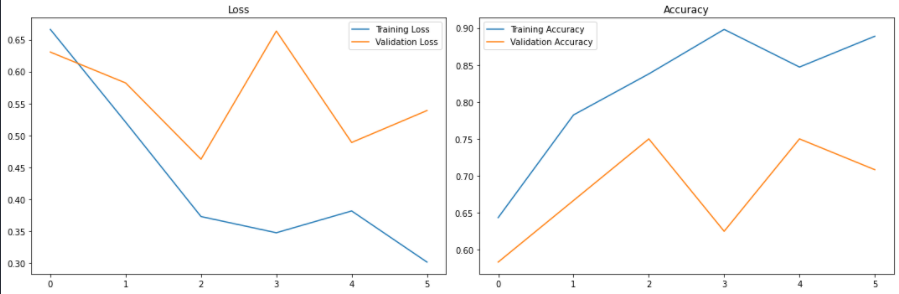
\includegraphics[scale=0.6]{Photos/v1.PNG}
\caption{Loss and Accuracy Graph of Version 1} \label{fig:ishan}
\end{figure}

Version 2 is a successor to version 1. Augmented data was used for training here. This version provides the best accuracy compared to other versions. However on seeing the loss graph it can be observed that there is a huge gap between train and validation loss indicating overfitting.
\begin{figure}[H]
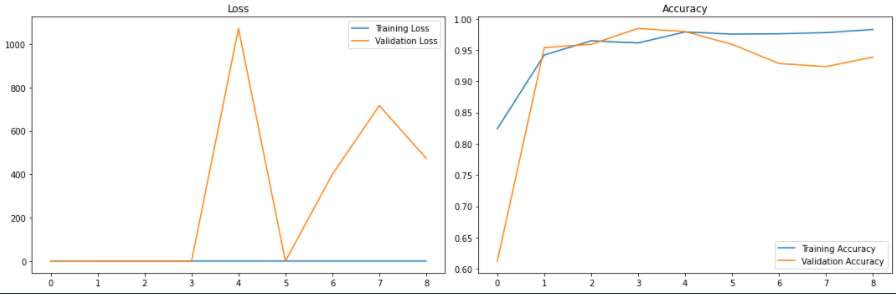
\includegraphics[scale=0.6]{Photos/v2.PNG}
\caption{Loss and Accuracy Graph of Version 2} \label{fig:ishan}
\end{figure}

Version 3 implemented a custom CNN model architecture. However the amount of images used were less, leading to a higher test loss and lower test accuracy.
\begin{figure}[H]
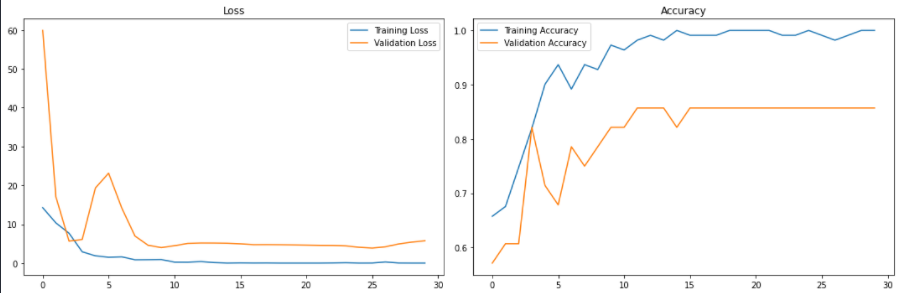
\includegraphics[scale=0.6]{Photos/v3.PNG}
\caption{Loss and Accuracy Graph of Version 3} \label{fig:ishan}
\end{figure}

Version 4 uses augmented data to try and resolve the issues faced from version 3. However on seeing the graphs it can be inferred that the model is overfitting.
\begin{figure}[H]
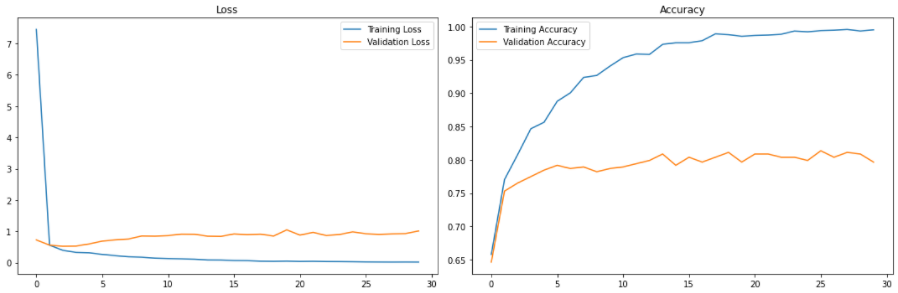
\includegraphics[scale=0.6]{Photos/v4.PNG}
\caption{Loss and Accuracy Graph of Version 4} \label{fig:ishan}
\end{figure}

Version 5 implements usage of callbacks to reduce this overfitting issue. The callbacks implemented are:
\begin{itemize}
    \item EarlyStopping : Early stopping is a method that allows user to specify an arbitrary large number of training epochs and stop training once the model performance stops improving on a hold out validation dataset.
    \item ModelCheckpoint : ModelCheckpoint is used to save a model or weights (in a checkpoint file) at some interval, so the model or weights can be loaded later to continue the training from the state saved.
\end{itemize}
Using callbacks test loss decreased, and test accuracy increased to an extent.
\begin{figure}[H]
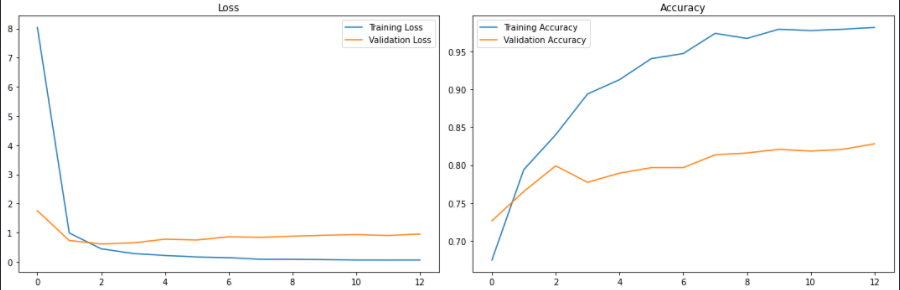
\includegraphics[scale=0.6]{Photos/v5.PNG}
\caption{Loss and Accuracy Graph of Version 5} \label{fig:ishan}
\end{figure}

To further improve the results obtained from version 5, volume of images used was increased, leading to the best performing model compared to the previous ones.
\begin{figure}[H]
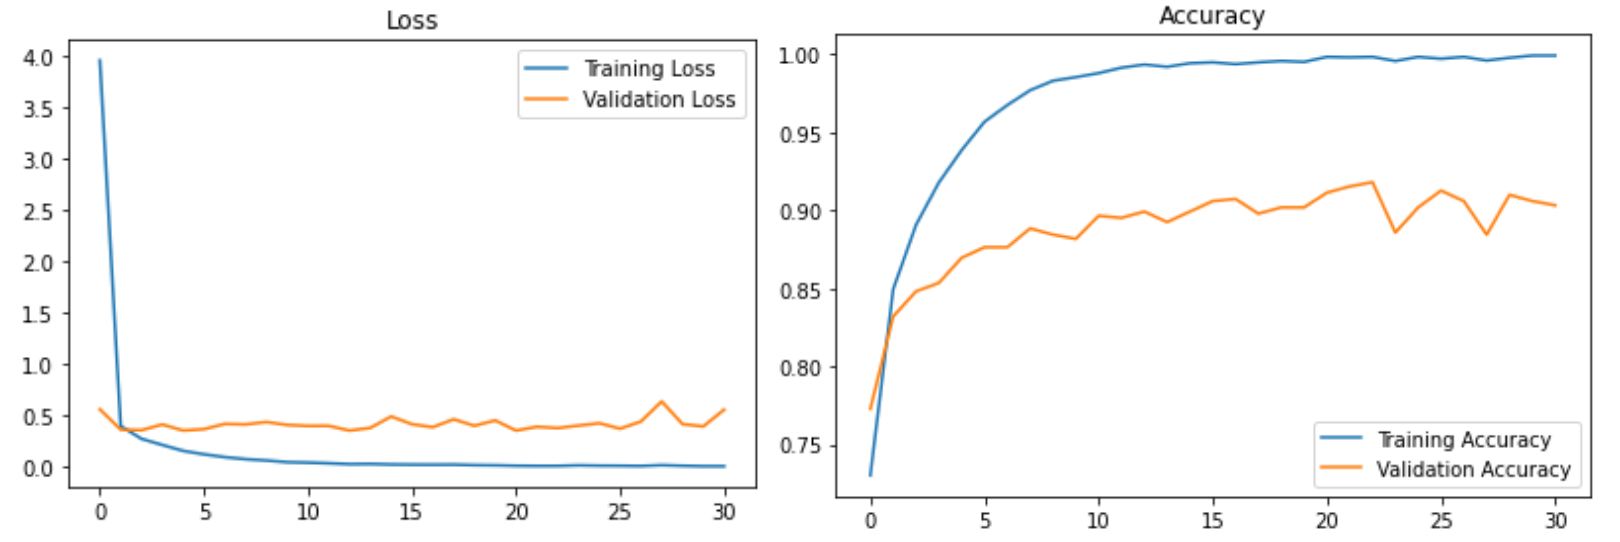
\includegraphics[scale=0.4]{Photos/v6.png}
\caption{Loss and Accuracy Graph of Version 6} \label{fig:ishan}
\end{figure}
    
\section{Manual Test Results}
In Manual Testing we use images from the third dataset to test the model on individual images. The images from third dataset have not been used to training of the model at any point; hence it acts as unbiased data. The results from the manual testing are as follows:
\begin{itemize}
    \item Tumor Present in the Brain:
        \begin{figure}[H]
        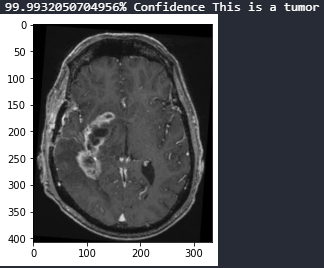
\includegraphics[scale=0.8]{Photos/Tumor_Manual_Result.PNG}
        \caption{Tumor Manual Testing Results} \label{fig:ishan}
        \end{figure}
    \item Tumor Absent in the Brain:
        \begin{figure}[H]
        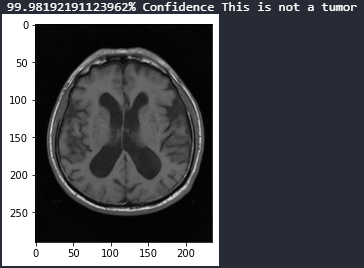
\includegraphics[scale=0.8]{Photos/Non_Tumor_Manual_Result.PNG}
        \caption{Non-Tumor Manual Testing Results} \label{fig:ishan}
        \end{figure}
\end{itemize}